\documentclass{article}
\usepackage[utf8]{inputenc}
\usepackage[top=1in]{geometry}
\usepackage{tikz}
\usetikzlibrary{circuits.logic.US,positioning,calc} 
\usepackage{graphicx}
\usepackage{booktabs}
\usepackage{amsmath}
\usepackage[colorlinks]{hyperref}
\title{CMOS circuit review}
\author{Vikas Dhiman for ECE275}
\newtheorem{prob}{Problem}
\newtheorem{example}{Example}

\newcommand{\bx}{\bar{x}}
\newcommand{\by}{\bar{y}}
\newcommand{\bz}{\bar{z}}
\newcommand{\bA}{\bar{A}}
\newcommand{\bB}{\bar{B}}
\newcommand{\bC}{\bar{C}}
\begin{document}
\maketitle
\section{CMOS gate review}

\begin{minipage}{0.45\linewidth}
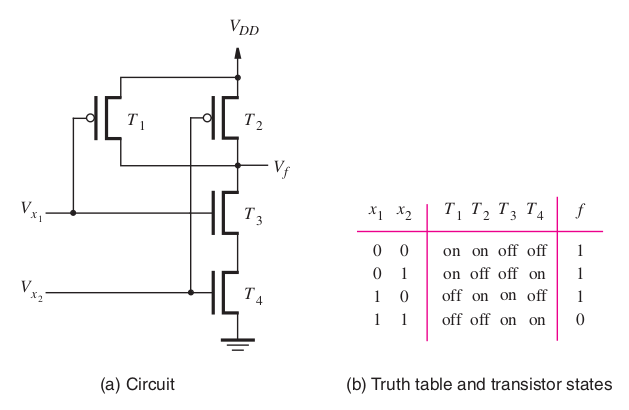
\includegraphics[width=\linewidth]{./fig/cmos-nand.png} \\
CMOS NAND gate
\end{minipage}
\begin{minipage}{0.45\linewidth}
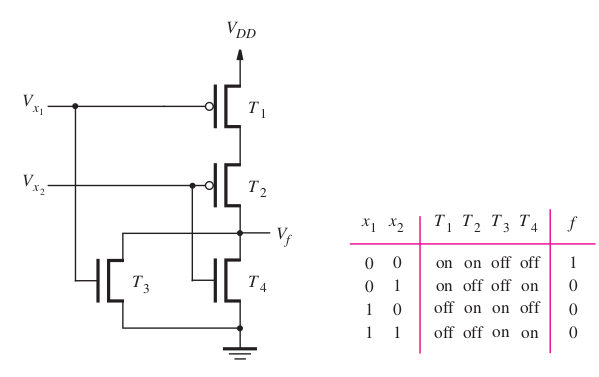
\includegraphics[width=\linewidth]{./fig/cmos-nor.png} \\
CMOS NOR gate
\end{minipage}\\
\begin{minipage}{0.45\linewidth}
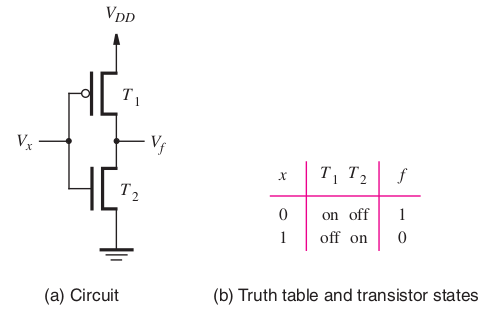
\includegraphics[width=\linewidth]{./fig/cmos-not.png} \\
CMOS NOT gate
\end{minipage}
\begin{minipage}{0.45\linewidth}
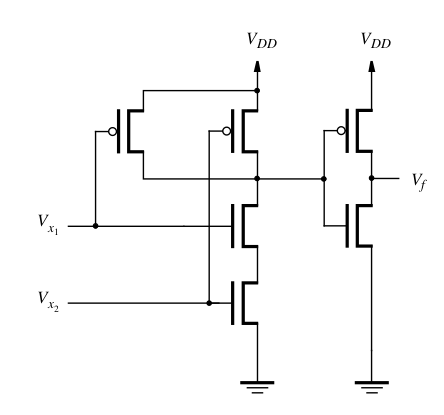
\includegraphics[width=\linewidth]{./fig/cmos-and.png} \\
CMOS AND gate
\end{minipage}


\begin{example}
  Derive the  CMOS complex gate that implements
  $f = \overline{x_1 x_2 + x_3 x_4 + x_5}$.
\end{example}

\begin{prob}
  Derive the  CMOS complex gate that implements
  $f = \bx_1 \bx_2 x_3 + \bx_1 x_2 \bx_3 + x_1 \bx_2 \bx_3 + x_1 x_2 x_3$.
\end{prob}

\end{document}